\documentclass[journal]{IEEEtran} 
\IEEEoverridecommandlockouts
% The preceding line is only needed to identify funding in the first footnote. If that is unneeded, please comment it out.
\usepackage{multirow}%,bigdelim}
\usepackage[hidelinks,draft]{hyperref} % draft is added to bypass issues seen with glossary terms broken up by line-breaks
\newcommand{\emaillink}[1]{\href{mailto:#1}{#1}}
\usepackage{url}
\usepackage{soul}
\usepackage{cite}
\usepackage{amsmath,amssymb,amsfonts}
\usepackage{mathtools}
\usepackage{siunitx}
\usepackage{xfrac}
% \usepackage{algorithmic}
\usepackage{graphicx}
\graphicspath{{figs/}}
\usepackage{tcolorbox}
\usepackage{textcomp}
\usepackage{xcolor}
\usepackage{siunitx}
\usepackage{xspace}
\usepackage[utf8]{inputenc}

% \usepackage{tablefootnote}
\usepackage[export]{adjustbox}

% tables
\usepackage{booktabs}
\usepackage{multirow}
\usepackage{makecell}

% Spacing
\usepackage[final]{microtype} % font expansion + protrusion

% \setlist[description]{leftmargin=\parindent,labelindent=\parindent}
\def\BibTeX{{\rm B\kern-.05em{\sc i\kern-.025em b}\kern-.08em
    T\kern-.1667em\lower.7ex\hbox{E}\kern-.125emX}}
\usepackage[textsize=tiny]{todonotes}
% \usepackage[textsize=tiny,disable]{todonotes}
% Maximize margin width to still barely see the sides of todonotes
\setlength{\marginparwidth}{1.3cm}

% Define a todolist for checkboxes
\makeatletter
\let\labelindent\relax
\makeatother
\usepackage[inline]{enumitem}
\newlist{todolist}{itemize}{2}
\setlist[todolist]{label=$\square$}
\usepackage{pifont}
\newcommand{\cmark}{\ding{51}}%
\newcommand{\xmark}{\ding{55}}%
\newcommand{\done}{\rlap{$\square$}{\raisebox{2pt}{\large\hspace{1pt}\cmark}}%
\hspace{-2.5pt}}
\newcommand{\wontfix}{\rlap{$\square$}{\large\hspace{1pt}\xmark}}

% \ifCLASSOPTIONcompsoc
%   \usepackage[caption=false,font=normalsize,labelfont=sf,textfont=sf]{subfig}
% \else
%   \usepackage[caption=false,font=footnotesize]{subfig}
% \fi
\usepackage[caption=false,font=footnotesize]{subfig}
\usepackage{titlecaps}
\usepackage{algorithm,algpseudocode}

%%%%%%%%%%%%%%%%%%%%%%%%%%%%%%%%%%%%%%%%%%%%%%%%%%
% Common macros
%%%%%%%%%%%%%%%%%%%%%%%%%%%%%%%%%%%%%%%%%%%%%%%%%%

\newcommand{\hsia}{H-Si(100)-2$\times$1\@\xspace}
\newcommand{\hsib}{H-Si(111)-1$\times$1\@\xspace}

% referencing labels
\newcommand{\fref}[1]{\figurename~\ref{#1}}
\newcommand{\tref}[1]{\tablename~\ref{#1}}
\newcommand{\secref}[1]{Section~\ref{#1}}
\newcommand{\eref}[1]{Eq.~\eqref{#1}} %\eqref provided by amsmath
\newcommand{\appenref}[1]{Appendix~\ref{#1}}

% in-text functions
\newcommand{\tsps}[1]{\textsuperscript{#1}}  % text superscripts
\newcommand{\tsbs}[1]{\textsubscript{#1}}  % text superscripts
\newcommand{\sref}[1]{\protect\subref{#1}}  % subfig referencing in main caption
\newcommand{\bpar}[1]{(\textbf{#1})}        % bolt text in parentheses

% To-do items
\newcommand{\TODO}[1]{\textcolor{red}{TODO: #1}}
\newcommand{\TODOlow}[1]{\textcolor{blue}{TODO: #1}}
\newcommand{\PLAN}[1]{
    \begin{tcolorbox}[colback=blue!30!white, % Background color
                      colframe=blue!60!black, % Frame color
                      boxsep=1pt, % Box padding
                      arc=2pt, % Corner rounding
                      boxrule=1pt] % Frame thickness
        \tiny
        #1
    \end{tcolorbox}
}
\newcommand{\OLD}[1]{\textcolor{lightgray}{#1}}

% math operators
\DeclareMathOperator\erf{erf}
\DeclarePairedDelimiter\ceil{\lceil}{\rceil}
\DeclarePairedDelimiter\floor{\lfloor}{\rfloor}
\newcommand{\vect}[1]{\boldsymbol{\mathbf{#1}}}
\DeclareSIUnit\angstrom{\text {Å}}

% Terms/math
\newcommand{\etal}{\textit{et al.}}

% \renewcommand{\baselinestretch}{0.99}

% Make \gls output with first letter of each word capitalized, not just first word
\usepackage{mfirstuc}

\makeatletter
\let\oldmakefirstuc\makefirstuc
\renewcommand*{\makefirstuc}[1]{%
  \def\gls@add@space{}%
  \mfu@capitalisewords#1 \@nil\mfu@endcap
}
\def\mfu@capitalisewords#1 #2\mfu@endcap{%
  \def\mfu@cap@first{#1}%
  \def\mfu@cap@second{#2}%
  \gls@add@space
  \oldmakefirstuc{#1}%
  \def\gls@add@space{ }%
  \ifx\mfu@cap@second\@nnil
    \let\next@mfu@cap\mfu@noop
  \else
    \let\next@mfu@cap\mfu@capitalisewords
  \fi
  \next@mfu@cap#2\mfu@endcap
}
\makeatother

\usepackage[acronym]{glossaries}

% Disable hyperlinks for glossary entries
\glsdisablehyper

% ML
\newacronym{ai}{AI}{artificial intelligence}
\newacronym{ml}{ML}{machine learning}
\newacronym{llm}{LLM}{large language model}
\newacronym{qat}{QAT}{quantization-aware training}
\newacronym{api}{API}{application programming interface}

% ML Accel
\newacronym{mvm}{MVM}{matrix--vector multiplication}
\newacronym{mxu}{MXU}{matrix multiply unit}
\newacronym{mac}{MAC}{multiply--accumulate}

% Atomic/Nanotech/Physics
\newacronym{stm}{STM}{scanning tunneling microscope}
\newacronym{afm}{AFM}{atomic force microscope}
\newacronym{set}{SET}{single-electron transistor}
\newacronym{bdl}{BDL}{binary-dot logic}

% Field-Coupled Nanocomputing
\newacronym{fcn}{FCN}{field-coupled nanocomputing}
\newacronym{sidb}{SiDB}{silicon dangling bond}
\newacronym{qca}{QCA}{quantum-dot cellular automata}
\newacronym{nml}{NML}{nanomagnetic logic}

% Devices
\newacronym{hal}{HAL}{hardware abstraction layer}
\newacronym{pi}{PI}{primary-input}
\newacronym{io}{I/O}{input/output}
\newacronym{adc}{ADC}{analog-to-digital converter}
\newacronym{cmos}{CMOS}{complementary metal-oxide-semiconductor}
\newacronym{cad}{CAD}{computer-aided design}
\newacronym{tpu}{TPU}{tensor processing unit}
\newacronym{alu}{ALU}{arithmetic logic unit}

% Architecture
\newacronym{pe}{PE}{processing element}

% EDA
\newacronym{rtl}{RTL}{register-transfer level}
\newacronym{eda}{EDA}{electronic design automation}
\newacronym{aig}{AIG}{and-inverter graph}

% fiction-specific algorithms
\newacronym{gold}{\emph{gold}}{graph-oriented layout design}
\newacronym{plo}{\emph{PLO}}{post-layout optimization}

% Others
\newacronym[longplural={figures of merit}]{fom}{FoM}{figure of merit}

\newcommand{\applyalwaysshortacros}{%
  \glsunset{ai}%
  \glsunset{ml}%
  \glsunset{llm}%
  \glsunset{cmos}%
  \glsunset{cad}%
}

\applyalwaysshortacros

% solve error: Page 1 has margin impositions
\def\IEEEtitletopspace{18pt}

\clubpenalty = 10000
\widowpenalty = 10000
\displaywidowpenalty = 10000

\begin{document}

\title{RTL-to-Atoms Synthesis of a Machine Learning Accelerator on Atomic-Scale Computers}

\author{Anonymous author(s)}

% Conference paper author list:
% \author{%
%     Samuel~S.~H.~Ng, %
%     Marcel Walter, %
%     Jan Drewniok, %
%     Simon Hofmann, %
%     Robert Wille, %
%     and Konrad Walus%
%     \thanks{This work was supported by the Natural Sciences and Engineering Research Council of Canada under Grant \mbox{RGPIN-2022-04830}.}%
%     \thanks{S.~S.~H.~Ng and K.~Walus were with the Department of Electrical and Computer Engineering, University of British Columbia, Vancouver, BC, Canada (\mbox{\{samueln, konradw\}@ece.ubc.ca}); M.~Walter, J.~Drewniok, S.~Hofmann, and R.~Wille were with the Chair for Design Automation, Technical University of Munich, BY, Germany (\mbox{\{marcel.walter, jan.drewniok, simon.t.hofmann, robert.wille\}@tum.de}). M.~Walter, S.~Hofmann, and R.~Wille were also with the Munich Quantum Software Company GmbH, Garching near Munich, BY, Germany. R.~Wille was also with the Software Competence Center Hagenberg (SCCH) GmbH, Hagenberg, O\"O, Austria.}%
% }

\section*{Extension Plan}

\subsection*{Main objectives}

Objectives that, together, satisfy \SI{50}{\percent} new contents rule:
%
\begin{todolist}
    \item[\done] Implement ripple-carry adder and array multiplier in Verilog with a wrapper that automatically generates N-bit versions
    \item[\done] Testbench the above for verification
    \item[\done] In the Processing Element, replace multiplication and accumulation operations with the optimized \glspl{alu} \textcolor{orange}{using Yosys's technology mapper}
    \item[\done] Synthesize and report changes
    \item \textcolor{orange}{Post-Yosys equivalence check (use PE-forward test bench)}
    \item[\done] \textcolor{orange}{Extend Verilogs to accept arbitrary width and activation bit-width settings}
    \item New table similar to DATE's table: report multiple algorithm combinations (e.g., ortho with and without PLO, FoM vs. uniform gates), \textcolor{orange}{test multiple bit-widths (W8A8, W4A4, W2A2)}, report FoM-informed results similarly
    \begin{itemize}
        \item Further study possible with gold with different cost metrics (e.g., area vs crossing vs area-crossing product etc.)
        \item Using CP as cost function might give us more squarish outputs
    \end{itemize}
\end{todolist}

\subsection*{Stretch goals}

\begin{todolist}
    \item Add half-adder gate to technology mapper
    \begin{itemize}
        \item \textcolor{orange}{Simon to look into adding HA to TM and synthesizing via \emph{gold}}
        \item \textcolor{orange}{Highly good-to-have if achievable without major roadblocks, do not sink too much time if there are significant hurdles!}
    \end{itemize}
    % \item \textcolor{red}{Demoted from main objectives:} Create multi-attempt averaged score benchmark set:
    % \begin{itemize}
    %     \item To clarify, this is an attempt at realizing that ``scientifically rigorous'' synthesis results comparison
    %     \item We can create a long-running script that makes $N$ attempts at deepsyn, TM to FoM-informed and uniform gates, $M$ attempts at \emph{gold} (if tractable). Since \emph{PLO} is deterministic we won't have to rerun that. This means $2 \cdot N \cdot M$ attempts in total. Missing anything?
    % \end{itemize}
    % \item If there's time, also try to improve the pin-routing area estimation (either by hand or by auto routing if available)
    % \begin{itemize}
    %     \item Marcel: can try using color routing in fiction
    %     \item Alternatively, Ben's planar placement \& routing algorithm
    % \end{itemize}
\end{todolist}


\maketitle

\begin{abstract}
%
\TODO{}
\vspace{20em}
% At a time when traditional CMOS technologies approach their fundamental scaling limits and artificial intelligence continues to escalate global computational demands, emerging post-CMOS technologies like \glspl{sidb} provide promising pathways towards energy-efficient computation.
% \glspl{sidb} offer atomic-scale precision and discrete charge control, enabling the realization of ultra-dense computational logic. However, manual layout design and verification have historically restricted the exploration and scalability of \gls{sidb}-based logic systems.
% To this end, this work demonstrates an automated, end-to-end \gls{eda} flow for designing and synthesizing a core component of a \gls{mxu} from high-level \gls{rtl} Verilog descriptions down to dot-accurate \gls{sidb} layouts. Leveraging recent advances in \gls{sidb}-focused \gls{eda} tooling, we demonstrate the first fully automated design flow capable of translating \gls{rtl} descriptions into manufacturable quantum-dot layouts. The proposed hierarchical Verilog approach addresses existing \gls{eda} constraints while facilitating comprehensive operational verification via test benches. Additionally, our design process incorporates reliability-focused \glspl{fom}, ensuring the selection of robust logic gates throughout synthesis.
% Our synthesized \gls{mxu} \gls{pe} layout represents a significant milestone in \gls{sidb} logic design, bridging previously manually-intensive workflows with scalable, automated methodologies. Despite achieving larger footprints than hand-crafted designs, the presented approach provides a valuable foundation for future optimization and widespread adoption of \gls{sidb}-based computing architectures.
%
\end{abstract}

% \begin{IEEEkeywords}
% Computer aided design, machine learning acceleration, quantum dots, silicon dangling bonds, simulation
% \end{IEEEkeywords}


\glsresetall
\applyalwaysshortacros

%%%%%%%%%%%%%%%%%%%%%%%%%%%%%%%%%%%%%%%%%%%%%%%%%%
% Introduction
%%%%%%%%%%%%%%%%%%%%%%%%%%%%%%%%%%%%%%%%%%%%%%%%%%
\section{Introduction} \label{sec:intro}

As \gls{cmos} scaling plateaus and \gls{ai} adoption accelerates, the resulting growth in global computing energy demand is driving strong interest in far more energy-efficient hardware and emerging computing technologies. Among these, \gls{fcn} has emerged as an appealing post-\gls{cmos} computing paradigm, in which local field interactions encode logic states in the position of charges~\cite{lent2003molecular,ardesi2024modeling} or in the magnetic polarity of nanomagnets~\cite{bernstein2005magnetic,giri2016modeling}, enabling both computation and signal transmission. Among the various physical implementations of \gls{fcn}, quantum dots made of \glspl{sidb} stand out as a promising platform due to their atomically precise fabrication~\cite{huff2017atomic, achal2018lithography, pitters2024atomically} and discretely controllable charge states~\cite{haider2009controlled, pitters2011charge}.

Motivated by the successful experimental demonstration of an \gls{sidb} \textsc{or} gate measuring just $\SI{5}{\nano\meter}\times\SI{6}{\nano\meter}$~\cite{huff2018binary}, specialized \gls{cad} tools and \gls{eda} frameworks have emerged to support \gls{sidb} logic exploration at multiple levels.
At the physical design level, \emph{SiQAD}~\cite{ng2020siqad} and an ecosystem of simulators~\cite{chiu2020poissolver,drewniok2024need,lambooy2026clustercomplete} have allowed researchers to design \gls{sidb} layouts and simulate their electrostatic ground states, enabling efficient exploration of logic structures and design rules at the gate and circuit level~\cite{vieira2022threeinput, bahar2020design, ahmadpour2023energyaware}, especially relative to experimental prototyping.
However, the fully manual design of these layouts remained a time-consuming process. More recently, automation introduced at multiple stages of the design flow has opened new pathways for large-scale \gls{sidb} logic implementations and studies. At the quantum-dot level, automated \gls{sidb} gate designers~\cite{lupoiu2022automated, drewniok2023minimal, drewniok2025quickcell} enabled the creation of standard-tile libraries~\cite{walter2022hexagons, ng2024unlocking}. With the addition of \gls{sidb} support in \emph{fiction}~\cite{walter2019fiction}, a state-of-the-art \gls{eda} framework for \gls{fcn} systems, higher-level exploration of \gls{sidb} applications has been made possible by automating synthesis from gate-level netlists down to dot-accurate \gls{sidb} layouts at scales impractical for manual design.

Prior to the maturity of \gls{sidb} \gls{eda} tools, application-scale research targeting \glspl{sidb} was scarce and relied on manually verified \gls{sidb} building blocks which were then extrapolated into system-level designs to estimate their behavior and implementation costs \cite{chiu2020poissolver, ng2023blueprint}. Among them was a quantized \gls{mxu} inspired by Google's \gls{tpu}~\cite{jouppi2017indatacenter} and optimized for \gls{sidb}'s architectural constraints~\cite{ng2023blueprint}, where the designer used simulation-proven \gls{sidb} logic components to approximate the area cost and performance figures.
To move toward practical implementation, an earlier conference version of this work was presented in \cite{ng2025building}, which realized the \gls{mxu} as a \gls{rtl} Verilog design using clocked registers as an abstract proxy for the underlying \gls{fcn} clocking behavior. With a workflow spanning multiple \gls{eda} frameworks, that study automatically synthesized the \gls{rtl} implementation into dot-accurate \gls{sidb} layouts, realizing an automated, scalable, and verifiable end-to-end \gls{sidb} design flow from \gls{rtl} descriptions through logic synthesis and optimization down to manufacturable quantum-dot layouts and establishing a first practical benchmark for \gls{sidb} application design and validation.

Despite this progress, the conference implementation left several aspects only coarsely explored: the choice of arithmetic units was left to logic synthesis frameworks, which does not take \gls{fcn}'s unique architectural preferences into account; weights and activations were fixed to a single 8-bit configuration, preventing any systematic study of how the \gls{rtl} and its layouts scale with precision; and it did not yet exploit emerging 2-input/2-output (2I2O) gate support in \emph{fiction} for more native arithmetic mappings\todo{delete this line if Marcel \& Simon's work on adding 2i2o support doesn't work out}.
This work therefore provides a substantial extension upon the original \gls{rtl}-to-atoms flow~\cite{ng2025building} by introducing \gls{fcn}-appropriate arithmetic building blocks within the logic-synthesis flow, generalizing quantization settings, and enabling a systematic study of the resulting architectural trade-offs. By exercising and extending state-of-the-art \gls{sidb} \gls{eda} tooling on a full \gls{mxu}, this work turns a one-off demonstration into a concrete framework for steering synthesis toward \gls{sidb}-appropriate arithmetic choices and for exposing how quantization and layout decisions shape the strengths and limitations of current tools.
The remainder of this manuscript is structured as follows. \secref{sec:background} reviews \gls{sidb} device operation and the relevant \gls{fcn} and \gls{eda} infrastructure; \secref{sec:related-work} summarizes prior \gls{sidb} \gls{mxu} designs; \secref{sec:methodology} details the hierarchical \gls{rtl} Verilog architecture and the \gls{rtl}-to-atoms synthesis flow; \secref{sec:results} presents the experimental protocol and synthesis results; and \secref{sec:conclusion-future-work} concludes with directions for future work.


% \TODO{Start the paragraph with a transition by briefly identify shortcomings of the conference paper.} This work provides a substantially extended treatment to the preceding conference paper \cite{ng2025building} by \TODO{new idea, new analysis, new results}. The remainder of the manuscript is structured as follows: \TODO{Section outline.}

% The rest of the manuscript is structured as follows: \secref{sec:background} covers background information on \gls{sidb} logic operation and design automation frameworks; \secref{sec:related-work} presents prior work on the \gls{sidb} \gls{mxu}; \secref{sec:methodology} describes our proposed methodology for designing the \gls{rtl} Verilog, test bench coverage for operational validation, and workflow for mapping the Verilog description down to dot-accurate layouts; \secref{sec:results} presents the synthesis results, comparisons between different settings and against past work, and discussions about their significance; \secref{sec:conclusion-future-work} concludes the manuscript and discusses potential future work.


%%%%%%%%%%%%%%%%%%%%%%%%%%%%%%%%%%%%%%%%%%%%%%%%%%
% Background
%%%%%%%%%%%%%%%%%%%%%%%%%%%%%%%%%%%%%%%%%%%%%%%%%%
\section{Background} \label{sec:background}

\begin{figure}
    \centering
    \subfloat[\gls{sidb} unit cell.]{
        \includegraphics[width=.25\linewidth,valign=c]{figs/bdl_demo.pdf}
        \label{sfig:sidb-logic-pairs}
    }\quad
    \subfloat[\emph{Bestagon} \textsc{nand} gate.]{
        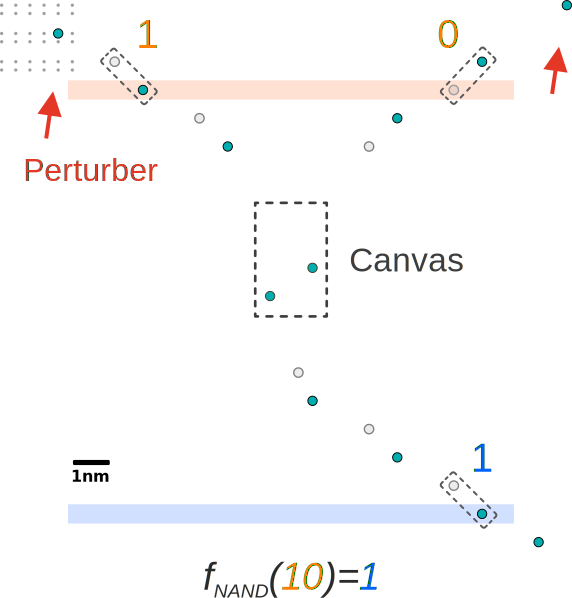
\includegraphics[width=.55\linewidth,valign=c]{figs/nand_10_bestagon_gate.pdf}
        \label{sfig:sidb-logic-hex-tile}
    }
    \caption{
        \TODO{Paraphrase.}
        \OLD{
        (\textbf{a}) A logic unit cell made of a pair of \glspl{sidb} sharing a single negative charge~\cite{huff2018binary} simulated in \emph{SiQAD}~\cite{ng2020siqad}. \textbf{Top:} the unit cell is illustrated without charges for readability; \textbf{middle:} unit cell simulated with charge, alongside an additional \gls{sidb} placed to the right (dubbed a \textit{perturber}), biasing the unit cell to take on logic state $0$; \textbf{bottom:} like above but with the perturber moved to the left, biasing the unit cell to take on logic $1$. Reprinted from~\cite{ng2023blueprint} with permission.
        (\textbf{b}) A \textsc{nand} gate from the \emph{Bestagon} library~\cite{walter2022hexagons} which defines standard locations for I/O pins and a canvas at the center which allows flexible placement of \glspl{sidb} to implement logic gates. Input pins are located at the top with input logic states set by input perturbers---a closer perturber pushes the input wire to the logic $1$ position, while a further one allows charges to take on logic $0$ state. The output is read out at the output pin located at the bottom. Adapted from~\cite{drewniok2025quicktrace} with permission.
        }
    }
    \label{fig:sidb-logic}
\end{figure}



\Glspl{sidb} can be manufactured on the surface of hydrogen-passivated Si(100)-2$\times$1 with the tip of a scanning-tunneling microscope \cite{achal2018lithography, huff2017atomic, pitters2024atomically}. Each \gls{sidb} is capable of holding discrete charge states, including negative, neutral, or positive. In densely packed ensembles, the charge state of each \gls{sidb} is determined by their collective interaction, bulk doping levels, and external electrostatic influences~\cite{pitters2024atomically}.
Binary logic states can be encoded by the position of a charge shared among closely positioned \glspl{sidb}, as illustrated in \fref{sfig:sidb-logic-pairs}, enabling the realization of logic gates such as an experimentally demonstrated \textsc{or} gate with a footprint of only $5\times\SI{6}{\nm^2}$~\cite{huff2018binary}.
Further exploration of \gls{sidb} gate and circuit designs~\cite{bahar2020atomic, ahmadpour2023energyaware, vieira2022threeinput} was enabled by \emph{SiQAD}~\cite{ng2020siqad}, an open-source \gls{cad} tool and simulation environment for \gls{sidb} layouts. Building on these tools, the \emph{Bestagon} standard-tile library~\cite{walter2022hexagons} was introduced, featuring standardized \gls{io} pin locations and a central canvas on which \glspl{sidb} are placed to implement logic. A representative \textsc{nand} gate from this library is shown in \fref{sfig:sidb-logic-hex-tile}.
The \emph{Bestagon} library has allowed \emph{fiction}~\cite{walter2019fiction}, an \gls{eda} framework specialized for \gls{fcn} logic, to take gate-level netlists as input and synthesize dot-accurate, fabricable \gls{sidb} layouts~\cite{walter2022hexagons}, thus forming the backbone of this work.

\Gls{sidb} logic, like other \gls{fcn} families, uses spatially partitioned clock zones to enforce directed data flow~\cite{ng2020siqad, chiu2020poissolver}. Hanging or buried electrodes apply phase-shifted sinusoidal potentials that modulate the surface band bending and thereby the local charge density~\cite{chiu2020poissolver}. Adjacent electrodes are offset by \SI{90}{\degree} in phase, producing ``active'' regions where charges are present and computation occurs, separated by ``inactive'' regions that are effectively charge-free buffers. A simple, area-efficient arrangement places these clock zones in rows to support unidirectional, purely combinational logic~\cite{lent1997device,chiu2020poissolver}.
Interfacing with \gls{cmos} can be achieved by biasing inputs electrostatically via electrodes~\cite{chiu2020poissolver}, while outputs can be sensed using charge-sensitive devices such as single-electron transistors~\cite{fuechsle2012singleatom, prager2009integration, bohloul2017quantum}.

%%%%%%%%%%%%%%%%%%%%%%%%%%%%%%%%%%%%%%%%%%%%%%%%%%
% Related work
%%%%%%%%%%%%%%%%%%%%%%%%%%%%%%%%%%%%%%%%%%%%%%%%%%
\section{Related Work} \label{sec:related-work}

\begin{figure}
    \centering
    \includegraphics[width=0.95\linewidth]{figs/mxu.pdf}
    \caption{
        A 2D systolic array \gls{mxu} receiving quantized activations ($a$), weights ($w$), weight control signals ($C_w$), and partial sums ($s$). \Glspl{pe} inside the \gls{mxu} consist of a \gls{mac} unit, memory controller, and delay-line memory for weight storage. Signals propagate downward on the left side of the \gls{pe} (forward pass) and upwards on the right side (return pass).
        \TODO{Consistent font size \& weight for I/O pins.} \TODO{Improve color scheme.} \TODO{Rounded corners in the right.}
    }
    \label{fig:mxu-systolic-array}
\end{figure}

Related \gls{fcn} design flows have been developed for \gls{nml}. \emph{ToPoliNano}~\cite{riente2017topolinano} provides a \gls{cmos}-like, top-down flow from structural VHDL descriptions to in-plane \gls{nml} layouts with clocking-aware placement, routing, and performance analysis.
Complementing this, \emph{FUNCODE}~\cite{garlando2021funcode} infers VHDL netlists from custom \gls{nml} layouts, enabling device-to-system analysis of \gls{nml} circuits using HDL simulators. These works demonstrate mature \gls{fcn} \gls{cad} capabilities in the \gls{nml} domain.
In contrast, the present work targets atomic-scale \gls{sidb} logic, integrating \gls{sidb}-specific standard cells, robustness-driven technology mapping, and an \gls{mxu} \gls{pe} \gls{rtl} to obtain dot-accurate \gls{sidb} layouts for machine learning workloads\todo{Is this sentence trying to add too much detail to the ``in contrast'' examples? It would have made sense if this was at the end of the section but this is the beginning of the Related Work section with a lot more after}.

Before dedicated \gls{sidb}-aware \gls{eda} tooling became available, studies of \gls{sidb} applications were limited and largely depended on manual \gls{cad} prototyping with extrapolated area and latency estimates.
One such example was an \gls{sidb} \gls{mxu}~\cite{ng2023blueprint} for \gls{ml} acceleration, which mirrored design choices from Google's \gls{tpu}v1~\cite{jouppi2017indatacenter}: the matrix-vector multiplications underpinning \gls{ml} workloads were realized as 8-bit integer \gls{mac} operations to reduce computational cost, and both designs employed a systolic-array architecture relying on regular arrangements of \glspl{pe}---homogeneous logic modules that operate on their inputs and pass results to adjacent \glspl{pe}---to perform computation (\fref{fig:mxu-systolic-array}).
At the \gls{pe} level, the core operation is a \gls{mac}:
%
\begin{equation}
    s_{\text{out}} = s_{\text{in}} + (w \cdot a),
\end{equation}
%
where $s_\text{in}$ the incoming partial sum from the preceding \gls{pe}, $w$ is the stored weight, $a$ is the incoming activation, and $s_\text{out}$ is the updated partial sum.

In the implementation of~\cite{ng2023blueprint}, each matrix-multiplication job consisted of two primary phases:
%
\begin{enumerate*}
  \item \emph{preloading}, where weights ($w$) are loaded into the array from the top edge and transverse column-wise until each one arrives at the designated \gls{pe}, which stores them;
  \item \emph{computing}, where activations ($a$) are streamed from the left side and are multiplied with the stored weights and accumulated with partial sums; activations continue to transverse row-wise while partial sums transverse column-wise for further accumulation until they reach the array's bottom edge.
\end{enumerate*}
%
Additional input signals control the operating phase and the destination \gls{pe} index of each input weight.
At the \gls{pe} granularity, each \gls{pe} comprises two signal paths: a \emph{forward pass} containing the \gls{mac} and memory controller, and a \emph{return pass} that drives a weight bus upward to close the delay-line memory feedback loop and an activation bus to align activations with neighboring \glspl{pe}. As shown in \fref{fig:mxu-systolic-array}, both paths are purely combinational, enabling row-wise clocking on each path.
As row-wise clocking necessitates deep pipeline stages (\secref{sec:background}), at each clock cycle, different inputs can be interleaved to increase the computational throughput of the \gls{mxu}.

That work reported up to $10\times$ reduction in area cost and up to $10^8\times$ increase in power efficiency when compared against Google's \gls{tpu}v1~\cite{ng2023blueprint, jouppi2017indatacenter}. However, since the overall layout of the \gls{sidb} \gls{mxu} was extrapolated based on smaller logic components verified in simulation, the approximated nature means that it offers neither an exact \gls{sidb} layout that can be manufactured and tested, nor any verification on operational correctness. To address these shortcomings, this work applies recent \gls{sidb}-aware \gls{fcn} \gls{eda} techniques to implement the \gls{pe} in \gls{rtl} Verilog, confirm full pipelined interleaved operation at the \gls{pe}-level with test benches, and establish a flow that yields dot-accurate layouts, as detailed in the following section.\todo{Rephrase this to add emphasis on latest contributions new in the journal extension.}

%%%%%%%%%%%%%%%%%%%%%%%%%%%%%%%%%%%%%%%%%%%%%%%%%%
% Methodology
%%%%%%%%%%%%%%%%%%%%%%%%%%%%%%%%%%%%%%%%%%%%%%%%%%
\section{Methodology} \label{sec:methodology}

In this section, the \gls{rtl}-to-atoms design and synthesis approach adopted in this work is outlined.
In \secref{sec:methodology-verilog}, a hierarchical \gls{rtl} Verilog design of the \gls{sidb} \gls{mxu} is presented in which a strictly combinational \gls{pe} core satisfies \gls{eda} input constraints while a clocked wrapper preserves pipeline timing, permitting test-bench validation of interleaved operation. In \secref{sec:methodology-eda}, the \gls{rtl}-to-atoms flow is detailed alongside technology-specific improvements contributed by this work.

\subsection{\titlecap{\glsentrylong{mxu} in Hierarchical RTL}}\label{sec:methodology-verilog}

\begin{algorithm}[tbp]
\footnotesize
\caption{Forward Pass Logic in Processing Element}\label{alg:pe-forward}

\renewcommand{\algorithmicrequire}{\textbf{Inputs:}}
\renewcommand{\algorithmicensure}{\textbf{Outputs:}}

\begin{algorithmic}[1]
    \newcommand{\codecomment}[1]{\textit{\textcolor{gray}{// #1}}}
    \Require
    \Statex $\mathit{PE}_{y} \gets$ y-index assigned to each PE (constant per PE)
    \Statex $m \gets$ PRELOAD (0) or COMPUTE (1) mode
    \Statex $w_\text{load} \gets$ weight to be loaded into memory
    \Statex $\mathit{PE}_{\text{target-}y} \gets$ target Y-index of $w_\text{load}$
    \Statex $s_\text{in} \gets$ input partial product
    \Statex $a \gets$ input activation
    \Statex $w_\text{mem} \gets$ weight loaded from delay-line memory

    \Ensure
    \Statex $s_\text{out}$: new partial sum
    \Statex $w_\text{mem-out}$: weight to write to delay-line memory

    \Procedure{ProcessingElementLogic}{}
    \State $p \gets \text{signed}(w_\text{mem}) \times \text{signed}(a)$\Comment{Multiply stored $w$ with $a$}
    \State $p_\text{signExtended} \gets \text{signExtend}(p, 24)$
    \State $s_\text{out} \gets s_\text{in} + p_\text{signExtended}$\Comment{Sum with partial sum}
    \If{$m = \text{PRELOAD}$ \textbf{and} $PE_{\text{target-}y} = PE_{y}$}
       \State $w_\text{mem-out} \gets w_\text{load}$\Comment{Update stored weight}
    \EndIf
    \State \Return $s_\text{out}$, $w_\text{mem-out}$, and other pass-through wires
    \EndProcedure
\end{algorithmic}
\end{algorithm}

To achieve this work's objectives, the \gls{rtl} implementation must satisfy the following requirements:
%
\begin{enumerate*}
  \item the \gls{rtl} implementation must obey \emph{fiction}'s requirement for gate-level netlists to be purely combinational; and
  \item operation of the pipelined \gls{pe} must be verifiable so that test benches can establish operational correctness, addressing the lack of formal verification in prior work~\cite{ng2023blueprint}.
\end{enumerate*}
%
Because the \gls{pe} includes forward and return paths that form an internal feedback loop, a direct \gls{rtl} implementation of the full \gls{pe} would conflict with \emph{fiction}'s requirement for purely combinational gate-level netlists.
To reconcile these constraints, this work adopts a hierarchical \gls{rtl} organization, separating the design into a combinational core and a clocked shell:
%
\begin{description}
  \item[Combinational core:] The \gls{pe}'s forward-pass logic is implemented in strictly combinational \gls{rtl}, as shown in Alg.~\ref{alg:pe-forward}, ensuring compatibility with subsequent synthesis steps.
  \item[Clocked shell:] A higher-level \gls{rtl} module captures the clocked operation of the full \gls{pe}, defining the component's input and output signals, pipelined internal signal steering, and synchronized signal timing for the return pass.
\end{description}
%
% As a \hl{workaround}\todo{Think of more positive work than ``workaround''}, this work proposes a hierarchical \gls{rtl} implementation:\todo{Can use the latex description environment with items ``Combinational core'' and ``Clocked shell'' (or with improved wording if you can think of any)} the \gls{pe}'s core logic in the forward pass is implemented in strictly combinational \gls{rtl} as shown in Alg.~\ref{alg:pe-forward} to ensure compatibility with subsequent synthesis steps; clocked operation of the full \gls{pe} is captured in a higher level \gls{rtl} defining the component's input and output signals, pipelined internal signal steering, and synchronized signal timing for the return pass.
Both the combinational core and the clocked shell are parameterized by the bit widths of weights and activations, \hl{enabling exploration of}\todo{Try to assign a purpose to this, e.g., for architectural learning? Characterizing scaling behavior? etc.} multiple configurations in \secref{sec:results}.

Correctness was validated with test benches across the stack, including both the combinational core and the clocked shell. These tests confirmed correct weight storage in preload mode and accurate \gls{mac} results in compute mode for representative input activations, stored weights, and partial sums.
In particular, interleaved inputs for concurrent \gls{mac} operation across all pipeline stages was also verified. All simulations were performed using Icarus Verilog~\cite{icarusverilog}. The logical correctness of the \gls{pe} was thus established prior to synthesis and physical mapping. The full open-source Verilog implementation is available on GitHub~\cite{githubsupplementary}\todo{Check code prior to final submission}.

\subsection{RTL-to-Netlist}\label{sec:methodology-eda}

After verifying the \gls{rtl}, the combinational \gls{pe} core is ready for the \gls{rtl}-to-atoms synthesis flow. At the high level, this includes an \gls{rtl} to gate-level netlist synthesis in order to produce a \emph{fiction}-compatible netlist, which is then ingested into \emph{fiction} for a multistep synthesis workflow, ultimately yielding a dot-accurate \gls{sidb} layout.\todo{The tone of this paragraph reads like a tutorial, we should make it sound more serioius/academic tone}

Starting with the \gls{rtl}-to-netlist stage, this work uses \emph{Yosys}~\cite{wolf2013yosys} to map arithmetic operators such as \mbox{accumulation (\texttt{+})} and \mbox{multiplication (\texttt{*})} into gate-level \glspl{alu}.
Absent explicit directives, \emph{Yosys} selects \gls{cmos}-optimized \gls{alu} implementations, which can underperform in \gls{fcn} because their strictly planar fabrics force gates and wires to share the same plane, altering the area and latency trade-offs \cite{kim2010multipliers}. To ensure technology-appropriate choices, this work supplies explicit gate-level descriptions of a ripple-carry adder and an array multiplier to the \emph{Yosys} technology mapper. These implementations have been shown to suit \gls{fcn} technologies thanks to their regular structure, which eases wiring congestion and limits the need for crossovers \cite{kim2010multipliers}.
The mapped netlist is then rewritten as an \gls{aig} with \emph{Yosys} and optimized with ABC's \textit{\&deepsyn}~\cite{brayton2010abc} strategy to reduce the network's node count.
Finally, the resulting gate-level netlist is validated against the \gls{pe}-core test benches to confirm functional correctness.

\subsection{Netlist-to-Atoms}

\subsubsection{\textit{fiction} Synthesis Flow}

The verified gate-level netlist is subsequently forwarded to \emph{fiction}~\cite{walter2019fiction}, whose \gls{fcn}-aware toolchain synthesizes it into an \gls{sidb} layout following the synthesis flow proposed by \cite{walter2022hexagons}:
%
\begin{enumerate}
  \item Technology mapping maps the \gls{aig} onto the \emph{Bestagon} gate library~\cite{walter2022hexagons}, exploiting the library's richer primitives to shrink the logic compared with an AND/INV-only basis.
  \item Placement and routing with the \textit{ortho}~\cite{walter2019scalable} or \gls{gold}~\cite{hofmann2024born} algorithm produces a layout on a Cartesian grid.
  \item \Gls{plo}~\cite{hofmann2023postlayout, hofmann2024late} reduces the footprint of the routed design.
  \item The Cartesian layout is projected onto a hexagonal grid~\cite{hofmann2023scalable} in preparation for applying the \emph{Bestagon} gates.
  \item SAT-based equivalence checking~\cite{walter2020verification} confirms that the optimized, hexagonalized layout preserves the gate-level behavior.
  \item The \emph{Bestagon} library~\cite{walter2022hexagons} is applied to the hexagonalized layout, yielding a dot-accurate \gls{sidb} implementation of the design.
\end{enumerate}
%
Over the course of this study, several pain points were identified with \emph{fiction}'s synthesis workflow, as well as opportunities to optimize tooling for \gls{sidb} synthesis\todo{This statement needs better framing/wording}.

\subsubsection{FoM-aware Technology Mapping}

\TODO{Add one-liner context that prior \emph{fiction} \gls{sidb} work treated all gates equally without conception of \glspl{fom}}.
Recent advancements in \gls{sidb} logic robustness studies have culminated in the creation of a unified cost function for \glspl{fom} for \gls{sidb} gates~\cite{drewniok2024unifying}. The cost function encompasses the dominant cost drivers---operational domain size~\cite{ng2020siqad, walter2023reducing}, thermal stability~\cite{drewniok2023temperature}, band-bending effects~\cite{pitters2011charge}, defect sensitivity~\cite{ng2024simulating, huff2019electrostatic, croshaw2020atomic}, and related factors---into a single score $\chi$. This work adopts $\chi$ as the objective for the technology mapper so that the flow prefers gates with higher predicted robustness, even when a less stable configuration might use fewer devices\todo{maybe rephrase the last sentence a bit, something like ``even if it comes at the cost of...''}. The resulting trade-offs are examined in \secref{sec:results}.

\subsubsection{Placement and Routing Improvements for SiDBs}

In \emph{fiction}, the foundational placement-and-routing framework was established predominantly for \gls{qca}'s Cartesian layout in 2DDWave clocking in mind~\cite{walter2019fiction}\todo{Polish sentence}; support for \gls{sidb} logic was realized through a \hl{reprojection}\todo{See if Marcel \& Simon are happy with this wording}~\cite{hofmann2023scalable}. An unintended side effect is that a layout which is smaller in Cartesian space\todo{relative to?} may become larger after hexagonalization\todo{Current writing doesn't make it clear why this would be the case. Should add a one-liner explaining hexagonalization's $45^\circ$ turn to establish context}. While there isn't any configuration in the \emph{orth} placement-and-routing algorithm which could compensate for this behavior, the more recent \gls{gold} algorithm~\cite{hofmann2024born} exposes a configuration for adjusting the cost function during placement and routing. \TODO{Mention what the default cost function was, introduce the proposed cost function that is more suitable of SiDBs and explain why.}

\TODO{If we're able to incorporate half-adder support in fiction and validate in gold, mention that here.}

\subsubsection{Hexagonalization Improvements}

The hexagonalization algorithm was also revised in this work to align the generated layouts with \gls{sidb} clocking expectations. The Cartesian layout prior to hexagonalization follows the 2DDWave clocking scheme~\cite{vankamamidi2008twodimensional}, placing primary inputs along the north and west borders and letting data advance diagonally in the southeast direction. Earlier hexagonalization routines~\cite{hofmann2023scalable} rotated this grid by $45^\circ$ and projected it onto the hexagonal lattice, which left many inputs recessed from the north edge. Those offsets lower the attainable throughput because some signals must be held across multiple cycles to rejoin the global timing. The updated flow stretches every input and output pins to the north and south boundaries after projection, producing layouts whose ports are time-aligned as they enter and exit the hexagonal fabric.

%%%%%%%%%%%%%%%%%%%%%%%%%%%%%%%%%%%%%%%%%%%%%%%%%%
% Experimental Results
%%%%%%%%%%%%%%%%%%%%%%%%%%%%%%%%%%%%%%%%%%%%%%%%%%
\section{Experimental Results}\label{sec:results}

\TODO{Section intro.}

\subsection{Experimental Protocol}

This comparative study aims to showcase the scaling behavior of various bit-width configurations for activations and weights, as well as the synthesis outcome under different technology mapper configurations and placement-and-routing algorithms.
Multiple bit-width configurations of the combinational \gls{pe}-core (\secref{sec:methodology-verilog}) are synthesized, including 2-bit, 4-bit, and 8-bit weights and activations, which are subsequently termed W2A2, W4A4, and W8A8, respectively. These selections correspond to widely studied quantized regimes for CNNs and Transformers where the dominant operations reduce to matrix multiplications that map directly onto an \gls{mxu} \cite{esser2020learnedstepsizequantization, banner2019post, jouppi2017indatacenter}.

\TODO{Variables that we test (FoM vs.~no FoM, ABC's c2rs vs.~deepsyn (optional), specify configurations for any fiction algs that have available configs or are probabilistic)}

% Original plan when we were going to do multi-run averages, but now I don't think we have to do that.
% \TODO{Describe our updated experiment protocol:}
% %
% \begin{enumerate}
%   \item Multi-run synthesis to gather mean statistics for probabilistic synthesis steps: number of attempts, random-seed handling, stopping criteria
%   \begin{itemize}
%     \item I think it also stands to reason that if a designer finds the post-optimization output to be bigger than the original input, then a human designer would discard those bigger outputs, therefore the reporting should also discard them too. But we can report on the discard rate.
%   \end{itemize}
%   \item Variables that we test (FoM vs.~no FoM, ABC's c2rs vs.~deepsyn, any fiction algs that have available configs or are probabilistic)
%   \item Reporting conventions: best, mean$\pm$std, \SI{95}{\percent} CI, success rate of probabilistic steps finding solutions (e.g., \emph{gold}), success rate of equivalence checks
% \end{enumerate}

% \begin{table*}
%     \centering
%     \caption{\OLD{Placed and Routed MXU Processing Element (Forward Pass)}}
%     \label{tab:pe-results}
%     \begin{tabular}{lccccccc}
%     \toprule
%     Experiment & Tiles ($w \times h$) & Physical dimensions (\si{\nm^2}) & Gates & Wires & Crossings & \glspl{sidb} \\
%     \midrule
%     All gates equally preferred & $515 \times 1043$ & $\num{30930} \times \num{35474}$ & \num{613}  & \num{120945} & \num{11880} & \num{1645777} \\
%     \gls{fom}-informed & $516 \times 1049$ & $\num{30990} \times \num{35678}$ & \num{607}  & \num{124048} & \num{11057} & \num{1685608} \\
%     \bottomrule
%     \end{tabular}
% \end{table*}

\subsection{Results and Discussion}

\begin{table*}
  \caption{Synthesized processing element in SiDB MXU}
  \centering
  \label{tab:pe-results}
  \begin{minipage}{\linewidth}
    \centering
    % \resizebox{\linewidth}{!}{
      \begin{tabular}{l@{\hskip 6pt}l@{\hskip 6pt}r@{\hskip 2pt}c@{\hskip 2pt}l@{\hskip 6pt}c@{\hskip 6pt}rcrr}
        \toprule
        \multirow[c]{2}{*}{\makecell[tl]{\textsc{Experiment}}} &
        \multirow[c]{2}{*}{\makecell[tl]{\textsc{Algorithm}}} &
        \multicolumn{5}{c}{\textsc{Tiles}} &
        \multicolumn{1}{c}{\textsc{Dimensions}} &
        \multirow[c]{2}{*}{\makecell[tl]{$|\text{SiDBs}|$}} &
        \multirow[c]{2}{*}{\makecell[tl]{\textsc{$t\,[s]$}}} \\
        \cmidrule(lr){3-7} \cmidrule(lr){8-8}
         & &
        $w$ & $\times$ & $h$ & $=$ & $A$ & \multicolumn{1}{c}{\textsc{W $\times$ H [\si{\nm} $\times$ \si{\nm}]}} &  & \\
        \midrule
        % --- Hand-designed baseline
        {Blueprint~\cite{ng2023blueprint}} & Manual approximation &
        -- & $\times$ & -- & $=$ & -- & \num{5000} $\times$ \num{8150} & -- & -- \\
        % --- IEEE-NANO baseline
        {Unspecified \glspl{alu}~\cite{ng2025building}} & \emph{ortho} + \emph{PLO} &
        \num{515} & $\times$ & \num{1043} & $=$ & \num{537145} & $\num{11877} \times \num{13622}$ & \num{1645777} & \num{91} \\
        % --- New
        \multirow[t]{2}{*}{\makecell[tl]{Optimized \glspl{alu}\\(This work)}} & \TODO{} &
        -- & $\times$ & -- & $=$ & -- & -- $\times$ -- & -- & -- \\
        & \TODO{} &
        -- & $\times$ & -- & $=$ & -- & -- $\times$ -- & -- & -- \\
        % --- DATE for our own reference, delete before submission
        % \multirow[t]{4}{*}{\makecell[tl]{BitNet b1.58 MXU\\(This work)}} & \emph{ortho} &
        % \num{154} & $\times$ & \num{372} & $=$ & \num{57288} & $\num{3559} \times \num{4861}$ & \num{263431} & $<\!1$\\
        % & \emph{ortho} + \emph{PLO} &
        % \num{98} & $\times$ & \num{233} & $=$ & \num{22834} & $\num{2269} \times \num{3046}$ & \num{178778} & \num{1078}\\
        % & \emph{gold} &
        % \num{87} & $\times$ & \num{190} & $=$ & \num{16530} & $\num{2016} \times \num{2485}$ & \num{133882} & \num{37}\\
        % & \emph{gold} + \emph{PLO} &
        % \num{86} & $\times$ & \num{184} & $=$ & \num{15824} & $\num{1993} \times \num{2407}$ & \num{132041} &\num{51}\\
        \bottomrule
      \end{tabular}
    % }
    \begin{minipage}{\linewidth}
      \footnotesize
      \vspace{0.5em}
      Runtime values are in seconds; $w$, $h$, and $A$ are the width, height, and resulting area (in tiles) of the layout, respectively; dimensions refer to the area footprint of the synthesized \gls{sidb} layout after applying the Bestagon gate library \cite{walter2022hexagons}; $|\text{SiDBs}|$ indicates the number of \glspl{sidb}. \TODO{Add columns: bit-width of weights and activations, FoM Awareness, HA Used (if applicable)} \TODO{Add footnote to Blueprint area that it's for the full PE, whereas the rest are only for the PE-forward path.}
    \end{minipage}
  \end{minipage}
\end{table*}

\OLD{Following the \gls{eda} workflow laid out in \secref{sec:methodology-eda}, we have successfully synthesized the \gls{rtl} Verilog description of the forward-pass \gls{pe} all the way down to a dot-accurate \gls{sidb} layout. We present the results in \tref{tab:pe-results}, which includes: the network dimension in terms of tile count, the physical dimension in \si{\nm^2}, as well as the counts of gates, wires, crossings, and \glspl{sidb} used in the layout. Note that in this table, every tile that is mapped to a wire in the final layout is counted as 1 wire, thus a single wire signal that spans across $10$ tiles would increment the value by $10$.
We can see that the layout resulting from \gls{fom}-informed technology mapping is slightly larger than the simpler alternative of treating all gates with equal preference, indicating that the technology mapper has indeed chosen costlier solutions that make use of more robust gates. This area trade-off comes with the benefit that \gls{sidb} gates with higher reliability metrics are more often employed in the layout, which can ultimately yield a more robust device. It is also important to note that the \gls{fom} values from~\cite{drewniok2024unifying} are derived from a specific variant of the \emph{Bestagon} library optimized under a particular set of physical conditions. Choosing different libraries or physical conditions may yield different trade-offs.
Also notable is that the original hexagonalization algorithm would have imposed a $\frac{1}{12}\times$ throughput limit compared to full throughput, a limitation that is now alleviated by extending the input pin wires (as discussed in \secref{sec:methodology-eda}) at no increase in area cost.}

\OLD{Although the synthesized \gls{sidb} layout only covers the forward pass of the \gls{pe}'s operation, it already represents all of the logic operations; the parts that are not included in the synthesized layout are purely for signal propagation, as described in \secref{sec:methodology-verilog}. We thus believe that there is value in comparing our results with the previously proposed blueprint~\cite{ng2023blueprint}. The blueprint reported an area footprint of $5000 \times \SI{8150}{\nm^2}$, which means that the area we've achieved is $\sim30\times$ higher than those estimated by the blueprint, and the gap would further widen if we were to synthesize the entire \gls{pe}. Why is there such a substantial increase in area compared to previous estimates?}

\OLD{We believe there are multiple contributing factors. Whereas the previously proposed blueprint used hand-designed components with fairly high logic gate density~\cite{ng2023blueprint, ng2020siqad}, this work uses the \emph{Bestagon} gate library which deliberately chose a large tile template to ensure sufficient separation between the logic canvas of neighboring logic tiles in order to minimize inter-gate interference~\cite{walter2022hexagons}. Furthermore, the blueprint study benefited from deliberately chosen multiplier and adder implementations that were, themselves, systolic array designs optimized for \gls{fcn} implementation. In this study, the choice of arithmetic unit implementation is completely left to Yosys and ABC's synthesis tools, which are optimized for traditional CMOS devices with very different architectural trade-offs. Furthermore, once we perform logic optimization with ABC, the boundaries of arithmetic elements get completely blurred, hindering the possibility of potential optimization algorithms that could benefit from such arithmetic knowledge.
Lastly, due to the large size of the netlist required by this application (in relation to other \gls{fcn} applications), it is computationally intractable to use the optimal placement and routing algorithms offered by \emph{fiction} such as the \textit{exact}~\cite{walter2018exact} and \textit{gold}~\cite{hofmann2024born} solvers. Instead, we had to rely on algorithms which prioritized runtime at the sacrifice of final area cost.
Nevertheless, the successful end-to-end design flow achieved by this study presents an encouraging demonstration of what state-of-the-art \gls{fcn} \gls{eda} tools can achieve on the \gls{sidb} platform, highlighting opportunities for further optimization.}


%%%%%%%%%%%%%%%%%%%%%%%%%%%%%%%%%%%%%%%%%%%%%%%%%%
% Future Work
%%%%%%%%%%%%%%%%%%%%%%%%%%%%%%%%%%%%%%%%%%%%%%%%%%
\section{Conclusion and Future Work}\label{sec:conclusion-future-work}

\OLD{In past studies, the design and verification of large-scale SiDB applications remained disconnected from their physical implementations, constrained by immature \gls{eda} tooling and manually-intensive workflows at the time~\cite{chiu2020thes, ng2023blueprint}. Enabled by recent advances in \gls{sidb}-focused \gls{eda} frameworks, this work presents the first automated, end-to-end design flow for implementing a processing element (\gls{pe}) of a \gls{sidb}-based \glsentrylong{mxu} designed specifically for machine learning acceleration.
Our hierarchical Verilog structure facilitates the synthesis of combinational components down to the \gls{sidb} level while enabling validation of the complete operational functionality through higher-level \gls{rtl} modules. By strategically separating core combinational logic from higher-level pipeline control, we successfully synthesized a majority of the \gls{pe}'s functionality into a dot-accurate \gls{sidb} layout, selectively omitting specific signal components from synthesis to accommodate \gls{eda} tooling restrictions. Although the synthesized layout exhibits a larger area compared to previous hand-crafted designs~\cite{ng2023blueprint}, our effort provides a concrete demonstration of automated design methodologies applied to \gls{sidb}-based circuits, and underscores opportunities for further optimizations in \gls{sidb}-specific \gls{eda} flows. Additionally, this study is the first to incorporate \gls{fom} considerations into \emph{fiction}'s technology mapping process, prioritizing gate reliability within synthesized layouts.}

\OLD{One limitation faced by this study is the lack of control over the implementation of fundamental arithmetic units such as adders and multipliers. Since the design trade-offs of \gls{sidb} logic differ significantly from CMOS designs, it is possible that our workflow for synthesizing \gls{rtl} Verilog to gate-level Verilog using established tools like Yosys and ABC is introducing unnecessary overhead due suboptimal implementation choices. Further improvements to this synthesis step, as well as further developments to \emph{fiction}'s placement and routing algorithms, can bridge the gap between synthesized layouts and expert-designs and incentivize further development of novel applications optimized for \glspl{sidb}.}


%%%%%%%%%%%%%%%%%%%%%%%%%%%%%%%%%%%%%%%%%%%%%%%%%%
% Bibliography
%%%%%%%%%%%%%%%%%%%%%%%%%%%%%%%%%%%%%%%%%%%%%%%%%%
\bibliographystyle{IEEEtran}
\bibliography{zotero_refs_2025,manual_refs}
% zotero_refs.bib: original bib file exported from Zotero
% zotero_refs_normalized.bib: modified bib file where author fields with >6 authors are converted to et al



\end{document}
